\documentclass[10pt]{article}
\usepackage[margin=1.5cm]{geometry}
\usepackage{booktabs,graphicx,amsmath}
\pagestyle{empty}
\begin{document}

\section*{Task 3: Why SafeDreamer Violates the Cost Limit}

\subsection*{Question}
SafeDreamer exceeds the cost threshold ($d=0$) on multiple SMAC maps.
Two candidate causes: (1)~world-model error (the model dreams it is safe when
it is not), or (2)~the Lagrangian multiplier $\beta$ rises too slowly to
enforce the constraint within the training budget.

\subsection*{Ruling out model error (Theorem~1, Task~5)}
The Theorem~1 empirical check (Task~5) shows that the world model is accurate
enough: the observed gap between real and imagined cost is 50--900$\times$
smaller than the theoretical bound~$\Delta$.  Model error is \emph{not} the
bottleneck.

\subsection*{$\beta$ dynamics diagnosis}
We pulled the Lagrangian multiplier (\texttt{Agent/Lagrangian}) and episode
cost (\texttt{main/cost}) timeseries from WandB for 5~SMAC maps at $d=0$
(3~seeds each).  Figures~\ref{fig:violators} and~\ref{fig:clean} show the
results.

\paragraph{Key finding: $\beta$ never converges.}
On all 5~maps, $\beta$ rises linearly throughout training and is still
climbing at 100k steps.  There is no plateau, no oscillation --- the
gradient-ascent update (lag-lr${}=10^{-5}$) is simply too slow.

\paragraph{Severity scales with map difficulty.}

\begin{table}[h]
\centering
\small
\begin{tabular}{lcccl}
\toprule
Map & $\beta$ at 100k & Cost at 100k & Initial cost & Verdict \\
\midrule
MMM      & 0.50  & $\sim$7--8 & $\sim$10 & worst --- $\beta$ rising but cost barely moves \\
1c3s5z   & 0.30  & $\sim$4--5 & $\sim$9  & bad --- cost dropping but far from 0 \\
8m       & 0.50  & $\sim$3    & $\sim$8  & medium --- cost dropping, $\beta$ still rising \\
3m       & 0.13  & $\sim$0.5  & $\sim$3  & mild --- almost working, needs more time \\
2m\_vs\_1z & 0.025 & $\sim$0.2  & $\sim$2  & best --- low cost, low $\beta$ needed \\
\bottomrule
\end{tabular}
\caption{$\beta$ and cost at end of training (100k steps, $d=0$, 3-seed mean).}
\label{tab:beta_summary}
\end{table}

On easy maps (2m\_vs\_1z, 3m), the initial cost is low so even a small $\beta$
suffices.  On hard maps (MMM, 1c3s5z, 8m), the initial cost is 8--10 dead
allies per episode; $\beta$ at 0.3--0.5 is not large enough to outweigh the
reward signal, so the policy keeps violating.

\subsection*{Conclusion}
The cost-above-threshold problem is a \textbf{Lagrangian convergence} problem,
not a model-accuracy problem:
\begin{itemize}
  \item The multiplier update is too slow relative to the 100k training budget.
  \item Given more training time, $\beta$ would eventually rise enough (the
        trend is monotonic), but SafeDreamer's sample efficiency advantage
        would be lost.
  \item A faster multiplier mechanism --- specifically PID-Lagrangian
        (Task~4) --- should fix this by adding proportional and derivative
        terms that respond to violation magnitude and trend, not just
        accumulated error.
\end{itemize}

\subsection*{Figures}

\begin{figure}[h]
\centering
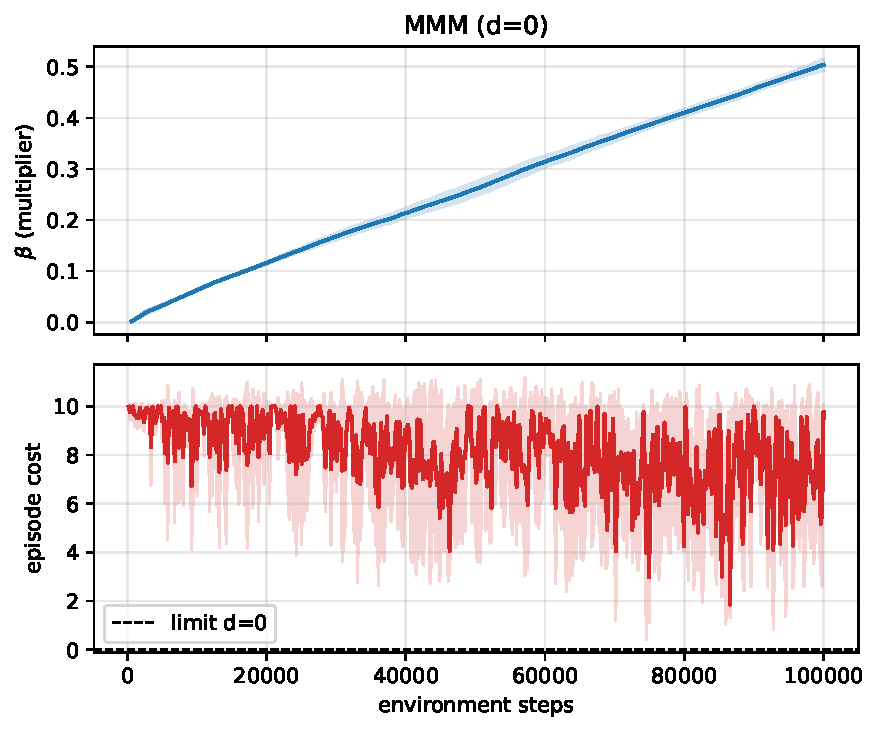
\includegraphics[width=0.32\textwidth]{figures/mmm_beta_dynamics.pdf}
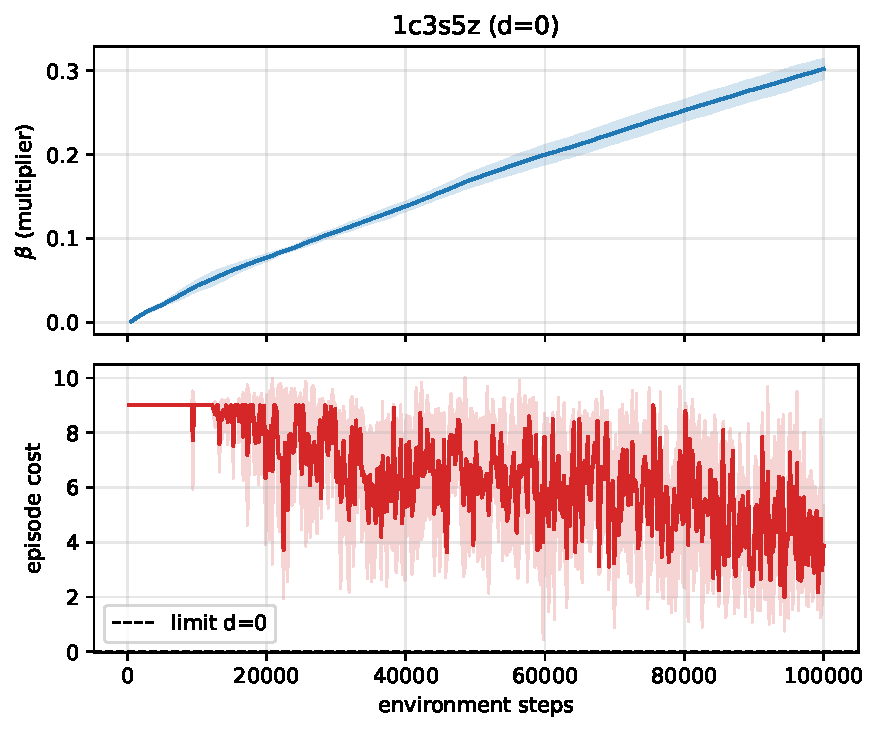
\includegraphics[width=0.32\textwidth]{figures/1c3s5z_beta_dynamics.pdf}
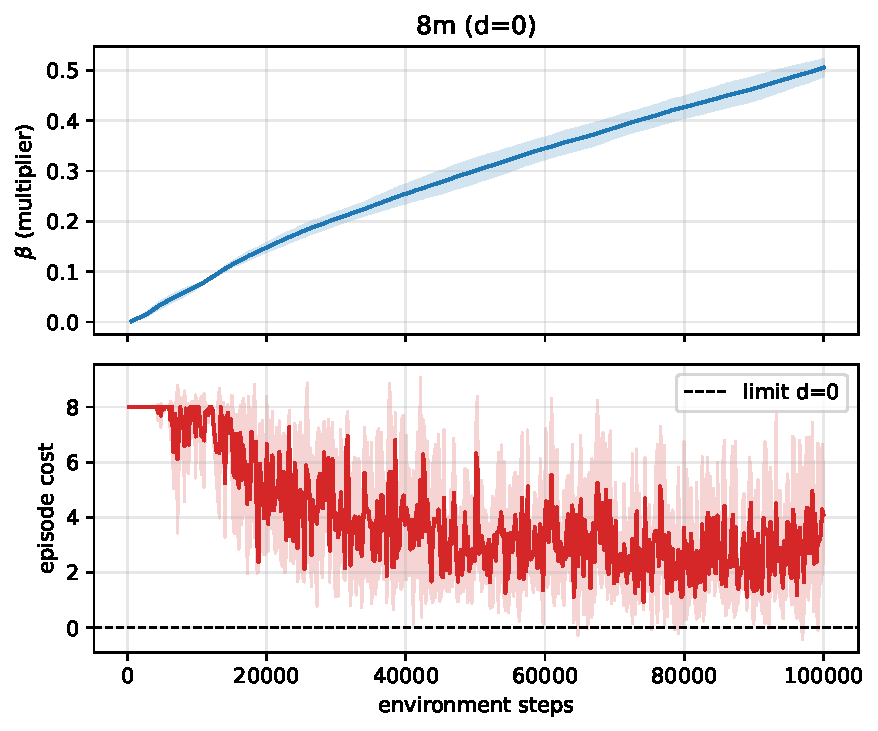
\includegraphics[width=0.32\textwidth]{figures/8m_beta_dynamics.pdf}
\caption{$\beta$ dynamics on violating maps (MMM, 1c3s5z, 8m).  $\beta$ rises
linearly; cost remains well above $d=0$ at 100k steps.}
\label{fig:violators}
\end{figure}

\begin{figure}[h]
\centering
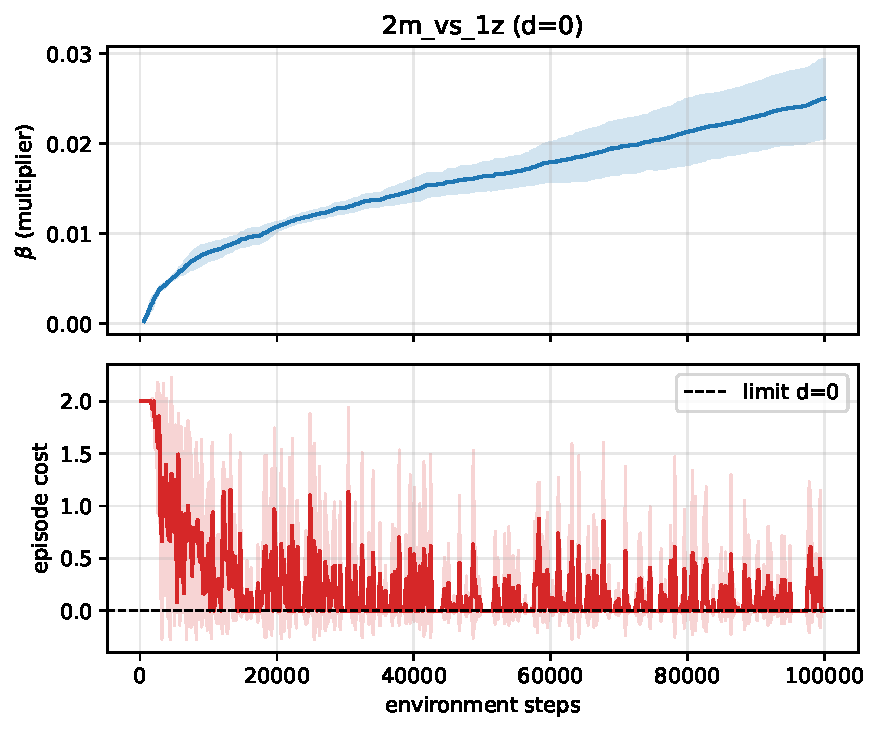
\includegraphics[width=0.32\textwidth]{figures/2m-vs-1z_beta_dynamics.pdf}
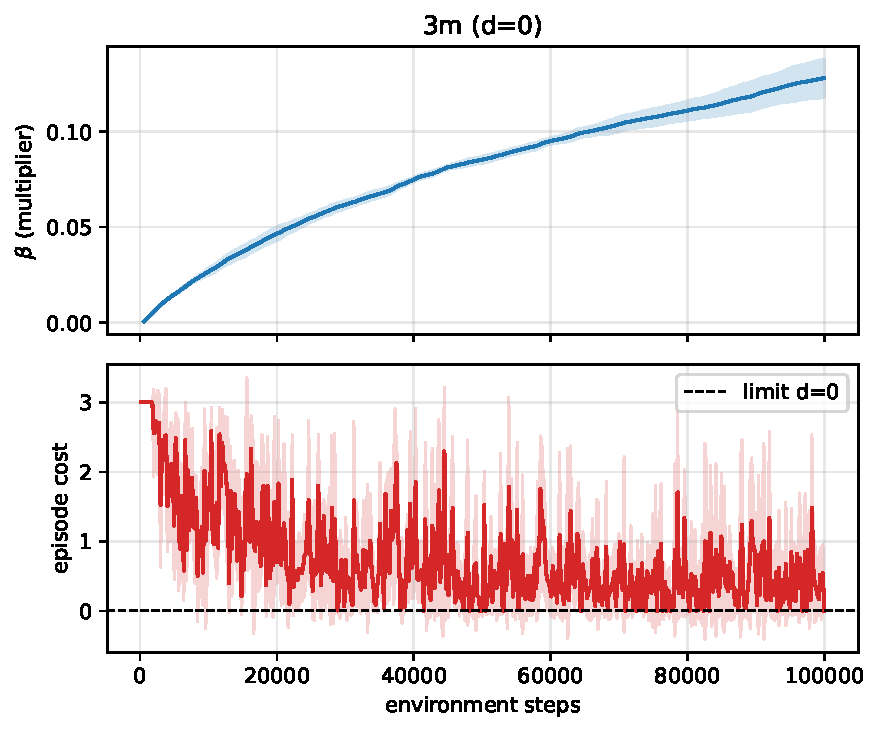
\includegraphics[width=0.32\textwidth]{figures/3m_beta_dynamics.pdf}
\caption{$\beta$ dynamics on clean maps (2m\_vs\_1z, 3m).  Lower initial cost
means a small $\beta$ is sufficient; cost approaches 0 by 100k.}
\label{fig:clean}
\end{figure}

\end{document}
